% Manuel Lippert - Paul Schwanitz
% Physikalisches Praktikum

% Teilaufgabe 2
% TODO: #23 FzV 2.2 @ManeLippert

\section{Das invertierte Pendel}
\label{sec:invertPendel}
Das invertierte Pendel erzeugt eine \textit{nichtlinearer} Schwingung. Dabei besitzt das Pendel eine unten fest eingespannte Blattfeder mit Federkonstante $k$, welche über zwei horizontal in der Höhe $h$ und der Auslenkung $x_h$ angreifende Spiralfedern mit Federkonstante $k_s$ un der Auslenkung $\hat{x}$ angetrieben wird. Am oberen Ende der Blattfeder lässt sich ein Zusatzgewicht $M$ anbringen und der Winkel $\theta$ beschreibt den Winkel zwischen der Tangenten an der Pendelspitze und dem Lot. Weiterhin bezeichnet die Pendellänge $L$ die Länge zwischen dem Anfang und Ende der Blattfeder, welche vom Winkel $\theta$ abhängt (siehe Abb: \ref{image:invertiertesPendel}).
\begin{center}
    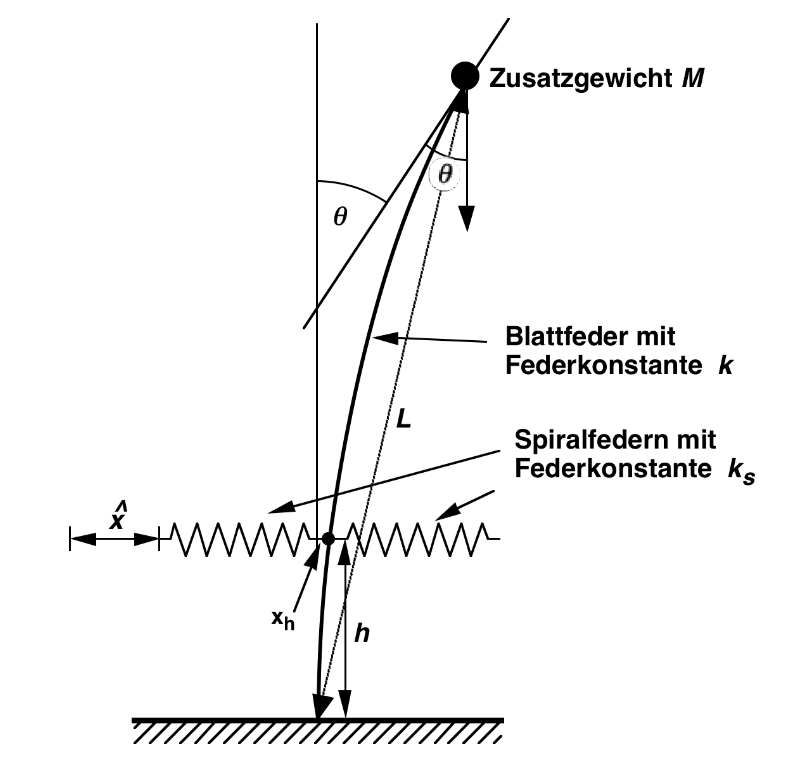
\includegraphics[scale=0.3]{invertiertesPendel.png}
    \captionof{figure}{Skizze invertiertes Pendel}
    \label{image:invertiertesPendel}
\end{center}
\subsection{Herleitung der Bewegungsgleichung}
\label{sub:bewegungsgleichung}
Die Bewegungsgleichung lässt sich über die wirkenden Drehmomente der Bauteile bestimmen:
\begin{gather*}
        \text{Pendel}~+~\text{Dämpfung}~+~\text{Blattfeder}~-~\text{Spiralfedern}~-~\text{Gewicht} = 0
\end{gather*}
\begin{gather}
    \Rightarrow [M(L(\theta))^2\ddot{\theta}]+[2c\dot{\theta}]+[k\theta]-[hk_s(x_h+\hat{x}\cos(\omega_at))]-[MgL(\theta)\sin(\theta)]=0
\end{gather}
Dabei bezeichnet $c$ die Dämpfungskonstante und $g$ die Erdbeschleunigung.\\
Im Folgenden wird die Pendellänge $L$ als konstant angenommen, obwohl dieser nicht konstant ist und von der Art der verwendeten Masse $M$ abhängt. Weiterhin wird die Auslenkung $x_h$ als vernachlässigbar klein angesehen und der Angriffswinkel der Spiralfedern wird als $\frac{\pi}{2}$ genähert, was bei genügend kleiner Höhe $h$ gegeben ist.
Daraus folgt die genäherte Form der Bewegungsgleichung:
\begin{gather}
    ML^2\ddot{\theta}+2c\dot{\theta}+k\theta-MgL(\theta)\sin(\theta)=hk_s\hat{x}\cos(\omega_at)=T_0\cos(\omega_at)
\end{gather}
Wobei $T_0$ als die Amplitude des periodisch angreifenden Drehmoments interpretiert werden muss. Hierbei ist noch zu erwähnen, dass durch die Näherungen die Lösung dieser Differentialgleichung nicht der tatsächlichen Trajektorien des Systems entsprechen, da diese stark von der Anfangsbedingung abhängen, dennoch ist eine globale Aussage über das Verhalten mit der genähreten Differentialgleichung möglich. \citep{Lueck}

\subsection{Symmetriebrechung}
\label{sub:symbrechung}
\textit{\textbf{Symmetriebrechung}} stellt den Übergang des Pendels von einem Monostabilen System ($M<M_k$) in ein bistabiles System ($M>M_k$) dar. Dieser Übergang geschieht bei einer \textit{kritischen Masse} $M_k=\frac{k}{gl}$, dabei ist die Bewegung des Pendels in beiden Fällen Unterschiedlich und muss deshalb getrennt betrachtet werden. \citep{Lueck}

\subsection{Schwingungsdauer in Abhängigkeit der Masse}
\label{sub:schwingungsdauer}
Bei einem nichtlinearen Pendel hängt, im Gegensatz zu einem linearen Schwingungsvorgang, die Eigenfrequenz $\omega_r$ von der Schwingungsamplitude $b$ ab $\Rightarrow \omega_r(b)$. Unverändert bleibt dennoch die Schwingungsamplitude $b(\omega_a)$ gegenüber der Resonanzkurve eines linearen Oszillators bei unterschiedlichen Anregungsfrequenzen $\omega_a$. \citep{Lueck}
\begin{itemize}
    \item[1.] $M<M_k$ (Schwache Nichtlinearität)\\
    Pendel ist nach (\ref{sub:symbrechung} monostabil.
    \item[2.] $M>M_k$
\end{itemize}

\subsection{Differenzier-Schaltung}
\label{sub:diffSchaltung}
\begin{center}
    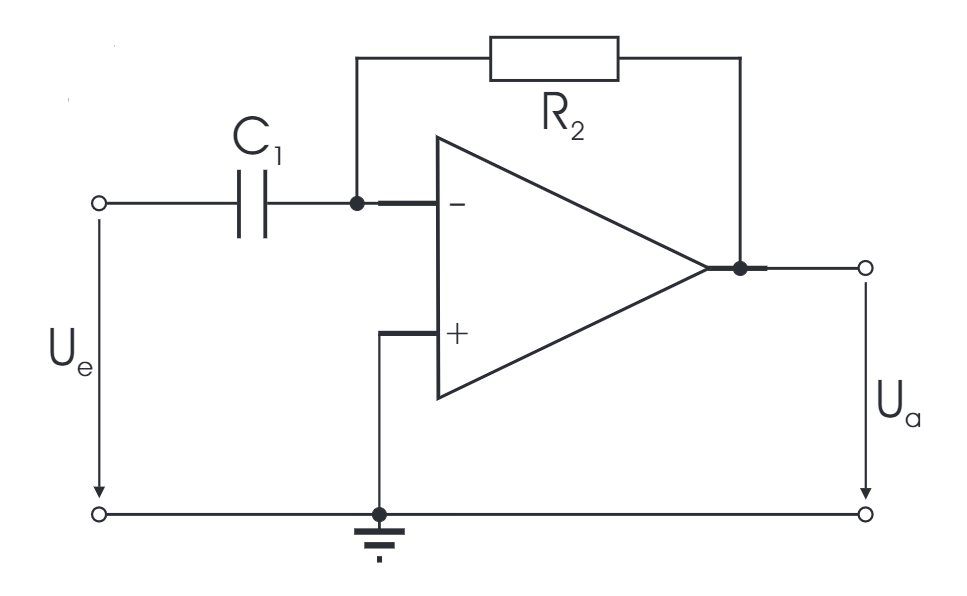
\includegraphics[scale=0.4]{diffOPV.PNG}
    \captionof{figure}{Differenzier-Schaltung}
    \label{image:diffOPV}
\end{center}
Bei einer Differenzier-Schaltung wird nur die die Änderung der Eingangsspannung zu einer Ausgangspannung verarbeitet. Dabei wird ein Kondensator am Eingang in Reihe und in Widerstand Parallel zwischen Eingang und Ausgang des Operrationsverstärker geschaltet (siehe Abb: \ref{image:diffOPV}). Durch den Kondensator fließt nur Strom, wenn sich die Eingangsspannung ändert, wobei die Ausgangsspannung proportional zur Änderungsgeschwindigkeit der Eingangsspannung ist. Durch den Operationsverstärker wird dann das Signal verstärkt, um dieses Signal besser über ein angeschlossenes Messgerät (z.B. Oszilloskop) betrachten zu können. \citep{electronik}
